\section{Experimental setup}
\label{sec:protocol}
\subsection{Molecular configurations and data splits}
The C16 pilot comprises 16 neutral, closed-shell
$\mathrm{C}_{16}\mathrm{H}_{34}$ parents: four base conformations,
each with an ordinary, torsional, bent, and contact configuration.
A base is an ideal all-trans chain together with a seeded Gaussian
displacement field of standard deviation 0.03~\AA\ per Cartesian
component. The same field is applied after each perturbation derived
from that base. Carbon--carbon and carbon--hydrogen bond lengths before
perturbation are 1.53 and 1.09~\AA, respectively, with tetrahedral angles.
The Atomic Simulation Environment (ASE) supports atomistic structure handling
\citep{larsen2017ase}.

Torsion rotates one connected side of a carbon--carbon bond; bending
rotates one connected side about a backbone vertex. Nonbonded contacts
are generated by folding consecutive torsions subject to topology and
clash constraints. Geometry checks reject changed bond topology,
inconsistent rigid operations, unacceptable bonds or angles, and
nonbonded clashes. Figure~\ref{fig:structures} shows the four actual
held-out C16 structures used in the pilot.

One base is assigned to each of the initial-training, calibration,
validation, and final-evaluation partitions, giving four structures per
partition. All structures derived from a base remain together.
This separation avoids direct sharing of a base displacement field
between partitions, but all four bases are closely related perturbations
of an all-trans chain; they are not a broad sample of equilibrium
conformations. A size-transfer check uses two
$\mathrm{C}_{32}\mathrm{H}_{66}$ parents from a single base, one torsional
and one contact configuration. It retains the extraction setting chosen
on C16 without reselection.

\begin{figure}[tb]
  \centering
  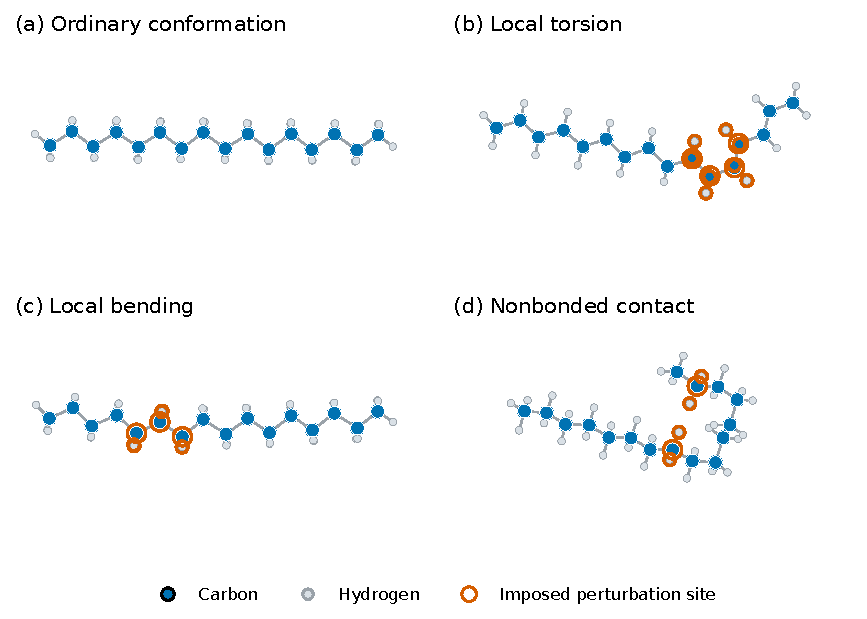
\includegraphics[width=\linewidth]{figures/fig02_configurations.pdf}
  \caption{Actual C16 final-evaluation structures: ordinary, torsional,
  bent, and folded-contact configurations. Carbon atoms are blue and
  hydrogen atoms light gray. Orange outlines indicate the imposed
  perturbation-site atoms from the generation record, not model-detected
  hotspots. Each structure is projected onto its own first two principal
  axes using the same spatial scale. These illustrations are generated
  from stored coordinates, not from a molecular image generator.}
  \label{fig:structures}
\end{figure}

\subsection{Reference calculations}
CP2K \citep{kuhne2020cp2k} supplies parent and fragment references using
the Perdew--Burke--Ernzerhof functional \citep{perdew1996pbe} with
DFT-D3 dispersion and Becke--Johnson damping
\citep{grimme2010d3,grimme2011d3bj}.
The basis is DZVP-MOLOPT-SR-GTH with GTH-PBE pseudopotentials;
the molecularly optimized basis construction is described in
Ref.~\citep{vandevondele2007molopt}.
Calculations use a singlet restricted description, 300~Ry cutoff,
50~Ry relative cutoff, and a self-consistent-field (SCF) tolerance
of $10^{-6}$. The initial solver uses orbital transformation with
a 100-iteration limit and a bounded retry policy.
Parents and fragments have identical electronic-structure settings.
An isolated WAVELET Poisson solver uses a cubic box enclosing the
structure with 6~\AA\ padding on each side.
The recorded cutoff probe gives a root-mean-square force difference of
approximately 0.006~\forceunit\ between 300/50 and 400/60~Ry; this is a limited
numerical probe, not a general convergence guarantee.

All reported reference jobs use one process with five OpenMP threads.
Cost is measured wall time multiplied by allocated cores and summed
over attempts, including failures and retries. This quantity is an
allocation measure, not a direct hardware-counter measurement of CPU
utilization. A reused label incurs no new computation, but an
acquisition arm is charged that label's historical measured cost
when comparing reference-data requirements.

\subsection{Potential and acquisition experiments}
GMD\_SGT trains a local equivariant potential with two blocks, scalar
dimension 32, representations $32\times0e+8\times1o$, eight radial
basis functions, and a 4~\AA\ local cutoff. No long-range term is enabled.
A primary model and two additional members form the committee.
The exploratory static-pool study uses at most 1500 training epochs,
batch size one, initial learning rate $2\times10^{-3}$, and patience
300. Energy-per-atom mean-absolute error and force RMSE have coefficients
0.1 and 1, respectively.

Four main arms acquire random local fragments, committee-ranked local
fragments, PHAL-selected local fragments, or full parents selected by
the PHAL policy. A fifth arm disables the LJ residual.
The candidate pool consists of the four calibration structures, with
candidate centers spaced along the chain. Each repetition starts with
four fully labeled training structures and has two acquisition rounds
of at most four labels. Seeds 11 and 23 define the two repetitions.
Full-parent acquisition deduplicates parent identities.
Force errors are measured on the four final-evaluation structures,
which are excluded from training and early stopping.

The completed comparison, denoted v2c in the archived records, is
post-hoc and exploratory. It evaluates every monitor stage on each
static configuration and fits the LJ feature without the lazy
light-stage gate. Configurations are scored independently against
calibrated statistics. The same final-evaluation set was inspected
during earlier exploratory versions, so it is not an untouched
confirmatory test set for the final protocol.

\subsection{Closed-loop and frozen-model trajectories}
The real-program closed-loop pilot starts from an ordinary initial-training
C16 structure at 300~K, with a 0.5~fs time step and a
Nos\'e--Hoover thermostat. Two 2000-step segments span 2~ps.
At most two labels per cycle and one per event are acquired, with
a 200-step cooldown. Fine-tuning uses at most 60 epochs, learning
rate $10^{-3}$, and patience 15.
Promotion requires validation force RMSE no greater than
1~\forceunit, at most 5\% regression, agreement of exported and
checkpoint forces within $10^{-4}$~\forceunit, and an engine check.
These thresholds were used for an integration demonstration, not a
qualification study of a reliable initial potential.

Initial and final frozen models are separately evaluated from the
same starting structure with three velocity seeds and 4000 steps
per seed. Frames are sampled every 20 steps; reported topology
fractions use steps 1000 through 4000, giving 151 frames per seed.
Topology retention means that the inferred bond set exactly equals
the parent bond set. Bonds are inferred at 1.3 times the sum of
ASE covalent radii, giving C--H and C--C cutoffs of 1.391 and
1.976~\AA, respectively. This is a fixed geometric diagnostic,
not an electronic bond-order calculation.
MD uses a periodic box large enough to separate molecular copies
relative to the architecture's nominal 16~\AA\ force-dependence
bound. Reference calculations remain nonperiodic.
All trajectory frames are checked for image separation.
